% vim:tw=72 sw=2 ft=tex
%         File: test2.tex
% Date Created: 2015 Feb 17
%  Last Change: 2015 May 16
%     Compiler: pdflatex
%       Author: joshua
\documentclass[10pt,a4paper]{article}
\usepackage{amsmath, amssymb}
\usepackage{amsthm}
\usepackage[utf8]{inputenc}
\usepackage[T1]{fontenc}
\usepackage[english]{babel}
\usepackage{graphicx}
\usepackage{mathrsfs} % gives me a font I need
\usepackage[document]{ragged2e} % flush everything left dont wory about
% the error

\DeclareMathOperator\arctanh{arctanh}
\DeclareMathOperator\sech{sech}


\newtheorem*{theorem}{Theorem}
\newtheorem*{corollary}{Corollary}

\theoremstyle{definition}
\newtheorem*{definition}{Definition}
\newtheorem*{example}{Example}

\everymath{\displaystyle}


\graphicspath{ {./images/} }

\begin{document}
%\title{Notes for Second Test}
%\author{Joshua Bailey}
%\maketitle
%\newpage

% Date 02.17.15. --------------------------  {{{
\marginpar{Date: 02.17.15.}
\begin{example}
  \[ (2x \sin y \cos y ) y' = 4x^2 + \sin^2y \]
  \[ v = \sin y \implies\]
  \[ \frac{dv}{dx} = \cos y \frac{dy}{dx} \]

  Thus, 
  \[ 2xvv' = 4x^2 + v^2 \text{ (hom),  } w = v/x \]
\end{example}

\section{population models}

  Recall that the most basic population model, \\ 
  assuming constant birth and death rates, is 

  \[ P' = kP \text{ (separable)  } \]

  Now, we give birth rates and death rates the \\
  following units: 

  \[ \beta(t) = \text{ birth rate } \frac{ \text{ \# of births at t }}{
  \text{ (unit of population at t)(unit of time) }} \]

  \[ \delta(t) = \text{ death rate } \frac{ \text{ \# of death at t }}{
  \text{ (unit of population at t)(unit of time) }} \]

  with this, for some small \( \Delta t \), 

  \[ P(t + \Delta t) \approx P(t) + \text{ ( \# birth rate at t - \# death rate at t) } \Delta t \implies   \]
  \[ = P(t) + \beta (t) P(t) \Delta t - \delta (t) P(t) \Delta t \]
  \[ \implies \frac{ \Delta P}{ \Delta t} =  \frac{P(t + \Delta t) -P(t)}{ \Delta
  t}  \approx ( \beta(t) - \delta(t) ) P(t)  \]

  using a diff model, the above suggest that 

  \[ \boxed{ P' = (\beta - \delta ) P} \]

  This is called the general population \\[5mm]

  Now, consider population with constant 
  death rate, say \( \delta_0 \), and with a birth 
  rate given by 

  \[ \beta = \beta_1 - \beta_0P \]

  In context, \( \beta_0 \text{ , } \beta_1 > 0 \) by (1),

  \begin{align*}
    P' &= ( \beta_1 - \beta_0 P -\delta_0 ) P \\
    &= ( \beta_1 - \delta_0 ) P - \beta_0 P^2 \\
    &= \beta_0 P  \left( \frac{ \beta_1-\delta_0}{\beta_0} -P \right)  
  \end{align*}

  which has form 
  \[ P' =  kP(M-P) \]
  \( k = \beta_0 > 0 \) and \( M = (\beta_1 -\delta_0)/ \beta_0  \) we
  see that in context, M>0 here (2) 
  is separable; as 
  \[ \frac{P'}{P(M-P)} =k \implies  \]
  \[ \int \frac{1}{P(M-P)}dP = kt + C \]
  Note that

  \[ \frac{1}{P(M-P)} = \frac{1}{M} \bigg( \frac{1}{M-P} +
  \frac{1}{P}\bigg) \]

  Thus, 

  \[ \frac{1}{M} (- \ln | M-P| + \ln|P|) = kt + C \implies  \]
  \[ \ln \bigg| \frac{P}{M-P} \bigg| = Mkt + C \]

  Now, \( P_0 = P(0) \) yields 

  \[ C = \ln \bigg| \frac{P_0}{M - P_0}\bigg|  \]
  Thus,

  \[ \ln \Big| \frac{P}{M-P} \bigg| = \ln \bigg| \frac{P_0}{M - P_0}\Big| + Mkt\]

  Hence, if \( P > M \) or \( P_0 > M \) then  

  \[  \frac{P}{M-P} = \frac{P_0}{M - P_0} e^{Mkt} \implies \frac{M}{P}
  -1 =  \frac{M - P_0}{P_0} e^{-Mkt}\]
  \[ \implies  \frac{M}{P} = \frac{P_0 + (M-P_0)e^{-Mkt}}{P_0} \]
  \[ \boxed{P(t) = \frac{MP_0}{P_0 + (M-P_0)e^{-Mkt}} } \]
  Notice that
  \[ \lim_{t \to \infty} P(t) = \frac{MP_0}{P_0} = M \]
  If \( P<M \), so that \( P_0 < M \), then
  \[ P' = kP(M-P) > 0 \]
  so, P is increasing to M \\[5mm]
  On the other hand, if \( P > M \), so \\
  that \( P_0>M \), then 
  \[ P' = kP(M-P) <0 \]
  so, P is decresing to M \\
  Since \( P(t) \to M \) in \\
  either case, in context,  \\
  \( M>0 \), \(  ( M = 0 \text{ \& } P>M \implies extinction) \). \\
  % }}}  

  % Date: 02.19.15. ----------------------------- {{{
  \newpage  
  \marginpar{Date: 02.19.15.}
  Recall: logistics population model 
  \[ P(t) = \frac{MP_0}{P_0 + (M - P)e^{-Mkt}} \]

  \begin{example}
    Page 88 Problem \# 22 \\
    \(M=100 \times 10^3 \) total population At \( t=0 \), half the
    population have heard a rumor, roughly the rumors increases by 1000
    people after 1 day 

    \[ P_0 = 50 \times 10^3 \text{ \&   } P(1) = 51 \times 10^3 \]

    we can solve for k

    \[ 51 \times 10^3 = \frac{(100 \times 10^3) (50 \times 10^3)}{ 50
    \times 10^3 + (100 \times 10^3 - 50 \times 10^3) e^{-Mk}} \]
    \[ \implies 51 = \frac{5000}{50 +50e^{-Mk}} = \frac{100}{1+e^{-Mk}} \]
    \[ \implies \frac{51}{100} = \frac{1}{1+e^{-Mk}} \implies  \]
    \[  1+ e^{-Mk} = \frac{100}{51} \implies  e^{-Mk} = \frac{100}{51} -1
    \implies \]
    \[ -Mk = \ln \bigg( \frac{100}{51} -1 \bigg) \]
    \[ \implies k= - \frac{\ln ( \frac{100}{51} - 1)}{10 \times 10^3} > 0 \]

    Therefore we can now solve \( P(t) = 80 \times 10^3 \) \\
    for t. \\

  \end{example}

\section{Doomsday/Extinction Model:} 

  Here we assume that 
  \[ \beta = kP, \text{  } k>0 \]
  \[ \text{ \& } \delta  = \delta_0 \]

  Thus, the gen pop ODE, \( P' = (\beta -\delta )P \), becomes 

  \begin{equation}
    \tag{1}
    \label{Model1}
    P' = (kP-\delta_0)P = kP(P-\delta/k )
  \end{equation}

  put \( M = \delta / k > 0 \),
  \eqref{Model1} becomes

  \begin{equation}
    \tag{2}
    \label{Model2}
    P' = kP(P-M)
  \end{equation}

  constant \eqref{Model2} with the logistics \\
  ODE: \( P' =kP(M-P) \) we 
  can solve \eqref{Model2}; it is separable. Thus,
  \[ \frac{P'}{P(P-M)}= k \implies  \]
  \[ \int \frac{1}{P(P-M)}dP = kt + C \]

  Note:

  \[ \frac{1}{P(P-M)} = \frac{1}{M}( \frac{1}{P-M}- \frac{1}{P}) \]

  Therefore 

  \[ \frac{1}{M}( \ln|P-M| - \ln P ) = kt + C \]
  \[ \implies \ln  \bigg| \frac{P-M}{P}\bigg| = Mk + C \]
  \[ \implies \frac{|P-M|}{P} = e^{Mkt+C} \]

  If \( P_0 = P(0) \) then 

  \[ C = \ln \bigg|\frac{P_0-M}{P_0}\bigg| \]

  so,

  \[ \frac{P-M}{P} = \frac{P_0-M}{P_0}e^{Mkt} \]

  Now, in any case 

  \[ \frac{P-M}{P} = \frac{P_0 - M}{P_0}e^{Mkt} \implies \]
  \[ 1 - \frac{M}{P} = \frac{P_0-M}{P_0}e^{Mkt} \implies  \]
  \[ \frac{M}{P} = \frac{P_0- (P_0 -M) e^{Mkt} }{P_0} \implies  \]
  \[ \boxed{P = \frac{MP_0}{P_0 + (M-P_0)e^{Mkt}} } \]

  contrast with logistic ODE soln: 

  \[ P = \frac{P_0M}{P_0 + (M-P_0)e^{-Mkt}} \]

  % }}}

  % Date: 02.23.15. ------------------------------  {{{
  \newpage
  \marginpar{Date: 02.23.15.}
\section*{With explosion/extinction modol}

  Notice that 

  \[ P>M \implies P'>0 \implies P \text{ is increasing; } \]
  \[ P>M \implies P'<0 \implies P \text{ is decreasing; } \]

  Now, if \( P>0 \), then P has a vertical 
  asymptote at \( t_0 \) such that. 

  \[ P_0 + (M-P_0)e^{Mkt_0} = 0 \implies \]
  \[ e^{Mkt_0} = \frac{P_0}{P_0 - M}>0 \implies \]
  \[ Mkt_0 = \ln \frac{P_0}{P_0-M} \]
  \[ \boxed{t_0 = \frac{1}{Mk} \ln \bigg( \frac{P_0}{P_0-M} \bigg)} \]

  which is the time of "doomsday," i.e., the explosion of the population 

  \[ \lim_{t \to t_0^-} P(t) = \infty \]

  On the other hand, if \( P<M \), then \( M-P_0>0; \) the

  \[ \lim_{t \to \infty} P(t) = 0 \]
  j
  This is to say, over time, extinction occurs. 

  % }}}

  % Date: 02.24.15. ----------------------------- {{{
  \newpage 

  \marginpar{Date: 02.24.15}
\section*{equilibuim solns and stability}

  Def. An autonomous ODE has the form 

  \begin{equation}
    \tag{1}
    \label{autonomous ODE}
    \frac{dx}{dt} = f(x) 
  \end{equation}

  Notice that the slope field in \eqref{autonomous ODE} is "independent"
  of t.

\section*{ Newtons law of cooling} 

  \[ T' = k(A-T) \text{ , } k>0 \]

  Recall:

  \[ \int \frac{1}{A-T}dt = \int kdt = kt + C \implies \]
  \[ -\ln |A-T| = kt +C \implies  \]
  \[ |A-T| = e^{-kt-C} \]

  where \( T_0 = T(0) \implies  \)

  \[ -C = \ln |A-T_0|  \] 

  thus, 

  \[ |A-T| = |A-T_0|e^{-kt} \implies \]
  \[ A-T = (A-T_0)e^{-kt} \implies \]
  \[ \boxed{T(t) = A + (T_0-A)e^{-kt} } \]

  Notice that 

  \[ \lim_{t \to \infty} = A \]

  Also, notice that \( T(t) \equiv A \),  i.e, \( T(t) = A \) for all t,
  in a soln to the autonomous ODE \( T' = k(A-T) \). this is  an example
  of an "equilibruim soln" \\[5mm] 

  \begin{definition}
   \( x(t) \equiv  C \in \mathbb{R} \) is an equilibrium soln to \( x' =
   f(x) \text{ iff } x(t) \equiv C \) is a soln to \( x' = f(x) \)
  \end{definition}

  \begin{definition}
   \( x = C \in \mathbb{R}  \) is a critical point of \( x' = f(x) \) iff \( f(c) = 0 \)
  \end{definition}

  Notice that we say that "x is a critical point" iff \( 0 = f(C) =
  \frac{dx}{dt} \), which is similar to use in calc I of  "critical pt." \\[5mm]

  Prop. \( x=C \) is a critixcal pt \\
  of \( x'=f(x) \iff x(t) \equiv  C \) \\
  is an equilibrium soln to \( x' = f(x) \) \\
  proof. easy. \\[5mm] 
  Def. \( C \in \mathbb{R} \) is a stable critical \\
  point of \( x' = f(x) \) iff C is a \\
  critical pt of \( x' = f(x)  \) and \\
  \[ \forall \epsilon >0 \text{  } \exists \text{  } \delta >0 \forall \]
  \[ |x_0 -C| < \delta  \implies |x(t) -C| < \epsilon  \]

\section*{Ex (Logistics Modle)}
  \[ P' = kP(M-P) \implies \]
  \[ P(t) = \frac{MP_0}{p_0 + (M - P) e^{-Mkt} } \implies  \]
  \[ \lim_{t \to \infty}P(t) = M \]

  Ex(Standard pop Model) 

  \[ P' = kP \implies P(t) = P_0 e^{kt}  \]
  Here \( P=0 \) is a critical pt; however, \\
  \( P=0  \) is not stable. 
  Notice that \( P' = kP(M-P)  \) has two \\
  critical pts, namely, \( P = 0 \) and \( P =M \). \\
  Here \( P(t) = M \) is stable, whereas, \( P(t) \equiv 0 \) is not \\
  stable.  \\[5mm]  
\section*{Ex(explosion/ extinction model)}
  \[ P' = kP(P-M) \text{ , } k, M>0\]
  \[ \implies P(t) = \frac{MP_0}{P_0 + (M-P_0)e^{Mkt}} \]
  Both \( P=0 \) and \( P=M  \) are \\
  critical pts. however, if \( P_0 > M \) \\
  then ? a stable, whereas \\
  if \( P_0 <M  \)then only \( P=0 \) \\
  is stable.
  \[ |x_0 - C| < \delta  \implies  \]
  \[ (x(t) -C) < \epsilon  \]

  % }}} 

  % Date: 02.25.15. ------------------- {{{
  \newpage 
  \marginpar{Date: 02.25.15.}
\section{Logistics Population Model with  Harvesting}

  Recall the Logistics Pop Model: 

  \[ P' = kP(M-P) \text{, }k \text{, } M>0  \]

  We now consider

  \[ P' = kP(M-P)-h \]

  where h is a constant, think: \( h>0 \implies \) harvesting; \\

  \[ h<0 \implies \text{ stocking } \]

  Notice that 
  \begin{align*}
  P' &= -kP^2 + kMP -h \\
   &= -k(P^2 -MP + h/k) \\
   &= -k(P-N)(P-H) 
  \end{align*}

  where

  \[ \text{ H,N  } = \frac{M \pm \sqrt{M^2 -4h/k}}{2} \]

  Here H and N are distinct reals if and only if \( M^2 -4h/k > 0 \iff
   M^2 >4h/k \iff h<kM^2/4 \). so, if \( h>0 \) and H, N are distinct
   and real, then 

  \[ 0 < h< \frac{kM^2}{4} \]

  Say, H<N. Notice that 

  \[ h>0 \implies \]
  \[ \sqrt{M^2 -4h/k} <  \sqrt{m^2} \implies  \]
  \[ M- \sqrt{M^2 - 4h/k} > 0 \]
  \[ \therefore 0<H \text{ ; where,  } 0< H < N  \]
  Now, "separating,"  yields that 
  \[ \frac{P'}{(P-H)(P-N)} = -k \implies \]
  \[ \int \frac{1}{(P-H)(P-N)}dP = -kt + C  \]
  Notice that 
  \[ \frac{1}{(P-H)(P-N)}= \bigg(\frac{1}{P-N} - \frac{1}{P-H}\bigg) \frac{1}{N-H} \]
  Thus, 
  \[ \ln \bigg| \frac{P-N}{P-H}\bigg| = -(N-H)kt + C \]
  If \( P_0 = P(0)  \) then
  \[  C = \ln \bigg| \frac{P_0-N}{P_0-H}\bigg| \]
  Hence \(  \big| \frac{P-N}{P-H}\big| = e^c e^{-(N-H)kt} = \big| \frac{P_0-N}{P_0-H}\big| e^{-(N-H)kt}\)
  Now, in any case, 
  \[ \frac{P-N}{P-H} =  \frac{P_0-N}{P_0-H} e^{-(N-H)kt}\]
  \[ \lim_{t \to \infty} \frac{P-N}{P-H} = \lim_{t \to \infty} \frac{P_0-N}{P_0-H} e^{-(N-H)kt}	 \]
  \[ \therefore \lim_{t \to \infty}(P-N) =0 \text{ or } \lim_{t \to
  \infty} (P-H) = \pm  \infty  \]
  Q: Is \( N<M \)? \\
  Q; \( P(t) =  \)?
  % }}}

  % Date: 02.26.15 ------------------ {{{
  \newpage
  \marginpar{Date: 02.26.15 }
  Recall: 
  \[ \frac{P-N}{P-H} =  \frac{P_0-N}{P_0-H} e^{-(N-H)kt} \implies \]
  \[ (P-N)(P_0-H) = (P-H)(P_0-N)e^{-(N-H)kt} \implies \]
  \[ P(P_0-H)-N(P_0-H) = P(P_0-N)e^{-(N-H)kt} - H(P_0-N)e^{-(N-H)kt}
  \implies \]
  \[ P(P_0-H-(P_0-N)e^{-(N-H)kt} ) = N(P_0-H) -H(P_0-N)e^{-(N-H)kt}
  \implies \]
  \[ \boxed{P(t) = \frac{N(P_0-H) -H(P_0-N)e^{-(N-H)kt}}{P_0-H-(P_0-N)e^{-(N-H)kt} }} \]
  \( \therefore \)
  \[ \lim_{t \to \infty} P(t) = \frac{N(P_0-H)}{P_0-H} = N \]
  Now, if \( 0<h<kM^2/4 \) then
  \[ 0<H<N<M \]
  For recall that
  \[ H,N = \frac{M \pm \sqrt{M^2-4h/k}}{2} \]
  so since \( h>0 \implies M^2-4h/k < M^2 \implies  \)
  \[ \sqrt{M^2-4h/k} < M \implies M + \sqrt{M^2-4h/k} < 2M \]
  \[ N = \frac{M + \sqrt{M^2-4h/k}}{2} < M \]
  Here 
  % this is to find when P(t) = 0
  \[ N(P_0-H) -H(P_0-N)e^{-(N-H)kt_E} = 0 \]
  which has a soln if \( P_0 < H \)

  % }}}

  % Date: 03.02.15 ------------------ {{{
  \newpage
  \marginpar{Date: 03.02.15 }
\section*{Vertical Motion with Air Resistance}
  Recall Newton's 2nd Law:
  \[ ma = \sum F_i \text{ (net forces) } \]
  Here \( a = v' = dv/dt \), \( F_G \) (force due to gravity) \\
  and \( F_R \) (force due to air resistance). Now, 
  \[ F_G = -mg \text{ \& } (F_R < 0 \iff v>0) \]
  where \( g \approx 9.8m/s^2 \) Empirically, 
  \[ F_R = kv^p  \]
  where \( 1 \leq p \leq 2 \text{ \& } k>0 \) \\
  two cases, namely \( p=1 \text{ \& } p=2 \). \\[5mm]
  \( p=1 \) Here, we have that 
  \[ mv' = F_G + F_R \implies \]
  \[ mv' = -mg-kv \]
  since \( F_R = -kv \). Notice that 
  \[ \text{ (1) } v' = -g- \frac{k}{m}v \]
  \[ = -( \frac{k}{m}v +g) \]
  Also, notice that (1) is a 1st order linear ODE, 
  \[ v' + \frac{k}{m}v = -g \]
  where \( \rho = k/m \), called the drag constant. Thus 
  \[ v'= (\rho v + g) \implies \]
  (sup)
  \[ \frac{v'}{\rho v + g} = -1 \implies \int \frac{1}{\rho v +g} dv = -t
  +c \]
  \[ \implies \frac{1}{\rho} \ln |\rho v +g | = - t + c \]
  \[ \implies  \ln |\rho v +g | = -\rho t + c \]
  \[ c = \ln | \rho v_0 + g| \]
  \[ |\rho v +g | = | \rho v_0 + g| e^{-\rho t } \]
  \[ \rho v + g = | \rho v_0 + g| e^{-\rho t }  \implies\]
  \[ \boxed{ v(t) = \frac{1}{\rho} ((\rho v_0 + g )e^{-\rho t} -g )} \]
  Notice that \( \lim_{t \to \infty} v(t) = -g/\rho \); this is \\
  called terminal velocity. we denote this as 
  \[ v_{\tau} = -g/\rho \]
  Thus, 
  \[ \boxed{v(t) = (v_0 - v_{\tau}) e^{-\rho t} + v_{\tau}}  \]
  Now, 
  \[ x(t) = v_{\tau} t - \frac{1}{\rho} (v_0 - v_{\tau} ) e^{-\rho t} + c
  \implies\]
  \[ c = x_0 + \frac{1}{\rho} (v_0 - v_{\tau} ) \implies \]
  \[ \boxed{x(t) = x_0 + v_{\tau} t + \frac{1}{\rho} (v_0-v_{\tau}) (1 -
  e^{-\rho t }) } \]


  % }}}

  % Date: 03.03.15 ------------------ {{{
  \newpage
  \marginpar{Date: 03.03.15 }
  Recall that \(F_R = \pm kv^p  \), \( F_G = -mg \), and 

  \[ ma = \sum F = F_G + F_R \implies \]

  \[
  \tag{1}
  \label{eq:}
  v' = -g \pm \frac{k}{m} v^p = -g \pm \rho v^p
  \]
  where drag \( \rho = k/m \).\\
  p=2 there are 2 cases: \\
  (i) upward motion, \( F_R = -kv^2 \);\\
  (ii) downward motion, \( F_R = kv^2 \).\\[5mm]
  (i) Upward motion
  Here (1) becomes 
  \[ v' = -g-\rho v^2 = -g( \frac{\rho}{g} v^2 + 1) = -g((v \sqrt{
  \frac{\rho}{g}})^2+1) \]
  \[ \implies \int \frac{1}{(v \sqrt{\rho/g})^2 + 1} dv = -gt + c \implies \]
  \[ \frac{1}{ \sqrt{\rho/g}} \arctan(v \sqrt{\rho/g}) = -gt + c \implies
  \arctan  (v \sqrt{\rho/g}) = -t \sqrt{\rho g} + c \]
  \[ \implies c = \arctan (v_0 \sqrt{\rho/g}) \implies \]
  \[ v \sqrt{\rho/g} = \tan ( \arctan (v_0\sqrt{\rho/g}) - t \sqrt{\rho g})
  \implies\]
  \[ \boxed{v(t) = \sqrt{g/ \rho} \tan ( \arctan( v_0\sqrt{\rho/g}) - t
  \sqrt{\rho g})} \]
  Thus, 
  \[ x(t) = \sqrt{g/\rho} \frac{1}{ \sqrt{\rho g}} \ln | \cos(\arctan(v_0
  \sqrt{\rho/g}) -t \sqrt{\rho g})| + c \]
  \[ \implies = \frac{1}{\rho} \ln | \cos (\arctan(v_0 \sqrt{\rho/g} - t
  \sqrt{\rho g}| +c \]
  \[\implies c = x_0 - \frac{1}{\rho} \ln | \cos ( \arctan (v_0 \sqrt{\rho/g}))|
  \implies \]
  \[ \boxed{ x(t) = x_0 + \frac{1}{\rho} \ln \bigg| \frac{\cos(\arctan(v_0
  \sqrt{\rho/g}) -t \sqrt{\rho g}}{\cos (\arctan (v_0 \sqrt{\rho/g}))}
  \bigg|}  \]
  Here \( v(t) = 0 \) allows us to find \\
  time of max height, say \( t_m \)
  \[ \boxed{ t_m = \frac{1}{ \sqrt{\rho g}} \arctan(v_0 \sqrt{\rho /g})} \]
  (ii) Downward Motion
  \[ v' = -g+\rho v^2 = -g(1 - (v \sqrt{\rho/g})^2) \implies \]
  \[ \int \frac{1}{1 - (v \sqrt{\rho/g})^2}dv = -gt + c \] % Date: 03.04.15
  \marginpar{Date: 03.04.15 }
  \[ \frac{1}{ \sqrt{\rho/g}} \arctanh (v \sqrt{\rho/g} = -gt + c \implies
  \] 
  \[ \arctanh (v \sqrt{\rho/g} = - \sqrt{\rho g} t + c \implies \]
  \[ c = \arctanh ( v_0 \sqrt{\rho/g} ) \implies \]
  \[ v \sqrt{\rho/g} = \tanh ( \arctanh(v_0 \sqrt{\rho/g} - t \sqrt{\rho g}
  \implies\]
  \[ \boxed{ v(t) = \sqrt{g/\rho} \tanh ( \arctanh (v_0 \sqrt{\rho/g})-t
  \sqrt{\rho g})} \]
  \( \therefore \)
  \[ x(t)= \sqrt{g/\rho}( -\frac{1}{ \sqrt{\rho g}} \ln | \cosh ( \arctanh
  (v_) \sqrt{\rho/g} -t \sqrt{\rho g}) | + c\]
  \[ = -\frac{1}{\rho} \ln | \cosh ( \arctanh (v_0 \sqrt{\rho/g}) - t
  \sqrt{\rho g}| + c \]
  \[ \implies c = x_0 + \frac{1}{\rho} \ln | \cosh ( \arctanh (v_0
  \sqrt{\rho/g}))| \]
  \[ \therefore \boxed{ x(t) = x_0 - \frac{1}{\rho} \ln | \frac{\cosh
  (\arctanh (x_0 \sqrt{\rho/g} -t \sqrt{\rho g}}{ \cosh( \arctanh (v_0
  \sqrt{\rho/g}))}} \]
  \\[5mm]
  Thrm(Inverse Function trm). if \( f'(x) \neq 0 \) then \( f^{-1}\) is \\
  diff at \( y= f(x) \) and 
  \[ \frac{df^{-1}}{dy}(y) = \frac{1}{ \frac{df}{dx} (x) } \]
  \[ ( \frac{dx}{dy} = \frac{1}{ \frac{dy}{dx}}) \]
  where \( y = f(x) \iff x = f^{-1}(y) \) \\[5mm]
  Aside:
  \[ \text{ Ex } y = f(x) = \tanh x \implies \]
  \[ \frac{df^{-1}}{dy}(y) = \frac{1}{ \frac{df}{dx}(x)} =
  \frac{1}{\sech^2 x} = \frac{1}{1-\tanh^2 x} = \frac{1}{1-y^2} \]
  \\[5mm]
  \[ \text{ Ex } \int \tanh x dx = \int \frac{\sinh x}{\cosh x}dx \int
  \frac{1}{u} du = \ln|\cosh x | + c \]
  \( u = \cosh x \) \\
  \( u' = \sinh x \) \\[5mm]
  Aside: 
  \[ \cosh x = \frac{e^x - e^{-x} }{2} \]
  \[ \sinh x =\frac{e^x - e^{-x} }{2}  \]
  \[ \cosh'x = \sinh x \]
  \[ \sinh'x = \cosh x \]
  \[ \frac{f(x) \pm f(-x)}{2} \]

  \[ \text{ Ex }  \]

  % }}}

  % Date: 03.05.15 ------------------ {{{
  \newpage
  \marginpar{Date: 03.05.15 }
\section*{Escape Velocity}
  Recall Newton's Gravitational Law:
  \[ F = \frac{GmM}{r^2} \]
  where \( G \approx 6.67 \times 10^{-11}\). Let m be the \\
  mass of a projectile from a planet's surface \\
  of mass M of radius R. By 
  Newton's 2nd Law, 
  \[ ma = -\frac{GmM}{r^2} \implies \]
  \[ v' = -\frac{GM}{r^2} \]
  By the chain rule, 
  \[ \frac{dv}{dt} = \frac{dv}{dr} \frac{dr}{dt} = v \frac{dv}{dr} \]
  Thus, 
  \[ v \frac{dv}{dr} = -\frac{GM}{r^2} \text{ (separable) } \]
  \[ \int v dv = -GM \int r^{-2} dr \implies \]
  \[ \frac{v^2}{2} =  \frac{GM}{r} + c \implies \]
  \[ c = \frac{v_0^2}{2} - \frac{GM}{r_0} \]
  where \( r_0 = R \therefore \)
  \[ \frac{v^2}{2} = \frac{v_0^2}{2} - \frac{GM}{R} + \frac{GM}{r}
  \implies \]
  \[ v^2 = v_0^2 - \frac{2GM}{R} + \frac{2GM}{r} \]
  \[ > v_0^2 - \frac{2GM}{R} \]
  To "escape" the gravitational force \\
  of the planet, we must have that \\
  \( v>0 \) for all r. This happens if 
  \[ v^2 > v_0^2 - \frac{2GM}{R} > 0 \iff \]
  \[ v_0^2 > \frac{2GM}{R} \implies \]

\section*{Ex (p.109) \# 30}
  Newton's 2nd Law: 
  \[ ma = \text{ net forces } = F_e + F_m \]
  By Newton's Gravitational law, 
  \[ F_e = - \frac{GmM_e}{r^2} \text{ \& } \]
  \[ F_m = \frac{GmM_m}{(s-r)^2} \]
  \( \therefore \)
  \[ \frac{dv}{dt} = \frac{GMm}{(s-r)^2}- \frac{GM_e}{r^2} \]
  As before, 
  \[ v \frac{dv}{dr} = G( \frac{M_m}{(s-r)^2} - \frac{M_e}{r^2}) \]
  which is separable. Thus, 
  \[ \frac{v^2}{2} = G( M_m \int \frac{1}{(s-r)^2}dr - M_e \int
  \frac{1}{r^2}dr)  \]
  \[ = G( \frac{M_m}{s-r} + \frac{M_e}{r} + c \implies \]
  \[ \frac{v_0^2}{2} = G( \frac{M_m}{s-R} + \frac{M_e}{R}) + c \]
  \( \implies \)
  \[ \frac{v^2}{2} = G ( \frac{M_m}{s-r} + \frac{M_e}{r}) +
  \frac{v_0^2}{2} -G( \frac{M_m}{s-R}+ \frac{M_e}{R})
  \]
  % }}}

  % Date: 03.09.15 ------------------ {{{
  \newpage
  \marginpar{Date: 03.09.15 }
  Recall: 
  \[ ma = \sum F_i \text{ , } (r_0 = R) \]
  \[(r_0 = R) \text{ ,  } R \leq r \leq s \]
  where
  \[ F_e = - \frac{GmM_e}{r^2} \text{ \& } F_m = \frac{GmM_m}{(s-r)^2} \]
  thus, 
  \[ a = \frac{d^2r}{dt^2} = F_m + F_e = \frac{GM_m}{(s-r)^2}-
  \frac{GM_e}{r^2} \]
  By chain rule, 
  \[ \frac{d^2r}{dt^2} = \frac{dv}{dt} = \frac{dv}{dr} \frac{dr}{dt} = v
  \frac{dv}{dr} \]
  so, 
  \[ v \frac{dv}{dr} = \frac{GM_m}{(s-r)^2} - \frac{GM_e}{r^2} \text{
  (sep) } \]
  \[ \frac{v^2}{2} = \frac{GM_m}{s-r}+ \frac{GM_e}{r} + c \implies \]
  \[ c = \frac{v_0^2}{2} - \frac{GM_m}{s-R} - \frac{GM_e}{R} \]
  Hence, 
  \[ \frac{v^2}{2} \frac{GM_m}{s-r} + \frac{GM_e}{r}+ \frac{v_0^2}{2} -
  \frac{GM_m}{s-R} - \frac{GM_e}{R} \]
  we want \( v>0 \) % pic
  \[ a = 0 \implies \]
  \[ \frac{GM_m}{(s-r)^2} = \frac{GM_e}{r^2} \implies \]
  \[ (\frac{s-r}{r}) = \frac{M_m}{M_e} \implies \]
  \[ \frac{s}{r} -1  = \sqrt{M_m/M_e} \implies \]
  \[ \frac{s}{r} = 1 + \sqrt{M_m/M_e} = \frac{ \sqrt{M_e} \sqrt{M_e}}{
  \sqrt{M_e}} \]
  \[ r = \frac{s \sqrt{M_e}}{ \sqrt{M_m} + \sqrt{M_e}} \]
  Also, notice that 
  \[ v=0 \implies \]
  \[ \frac{v_0^2}{2} = \frac{GM_m}{s-r} + \frac{GM_e}{R} -
  \frac{GM_m}{s-R} - \frac{GM_e}{r} \]
  \( \therefore \)
  \[ v_0 = \sqrt{ 2G ( \frac{M_m}{s-R} + \frac{M_e}{R} - \frac{M_m +M_e +
  2 \sqrt{M_mM_e}}{s})} \implies \]
  \[ \boxed{ v_0 = \sqrt{2G ( \frac{M_m}{s-R} + \frac{M_e}{R} -
  \frac{1}{s}( \sqrt{M_m} + \sqrt{M_e})^2)}} \]

  Aside: 
  \[ \frac{1}{r} = \frac{ \sqrt{M_m} + \sqrt{M_e}}{s \sqrt{M_e}} \implies \]
  \[ \frac{M_m}{s-r} = \frac{M_m + \sqrt{M_mM_e}}{s} \]
  \[ \frac{M_e}{r} = \frac{M_e + \sqrt{M_mM_e}}{s} \]

  Aside:
  \[ r \sqrt{M_m}+ r \sqrt{M_e} = s \sqrt{M_e} \implies \]
  \[ r \sqrt{M_m} = \sqrt{M_e}(s-r) \implies \]
  \[ \frac{1}{s-r} = \frac{1}{r} \sqrt{ \frac{M_e}{M_m}} \implies \]
  \[ \frac{M_m}{s-r} = \frac{\sqrt{M_mM_e}}{r} \]

\section*{ Euler's Method}
  Given a slope field, \( y' = f(x, y) \), \\
  \& a specific soln to the initial \\
  value problem 
  \[ \frac{dy}{dx} = f(x, y) \text{ \& } (x_0, y_0) \]
  say \( y = y(x) \), then \( y(x_0) = y_0 \), \& \\
  Euler's method gives an algorithem \\
  for estimating the exact soln \( y = y(x) \) % pic was here
  \begin{flushleft}
    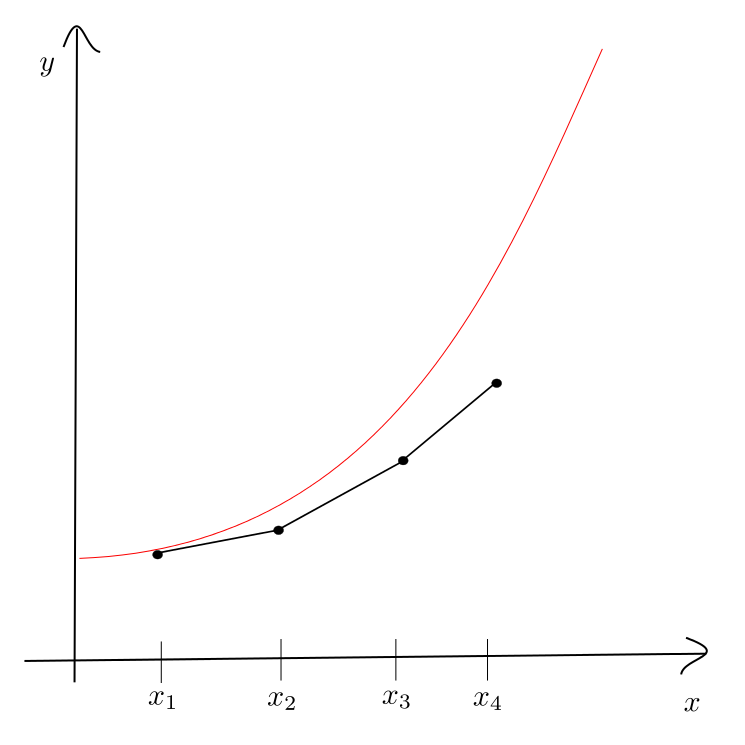
\includegraphics[scale=.3]{euler1}
  \end{flushleft}
  Find \( y_1 \text{ \& } y_{n+1} \) in general \\
  slope \( = f(x_0, y_0) \) \\
  \begin{flushleft}
    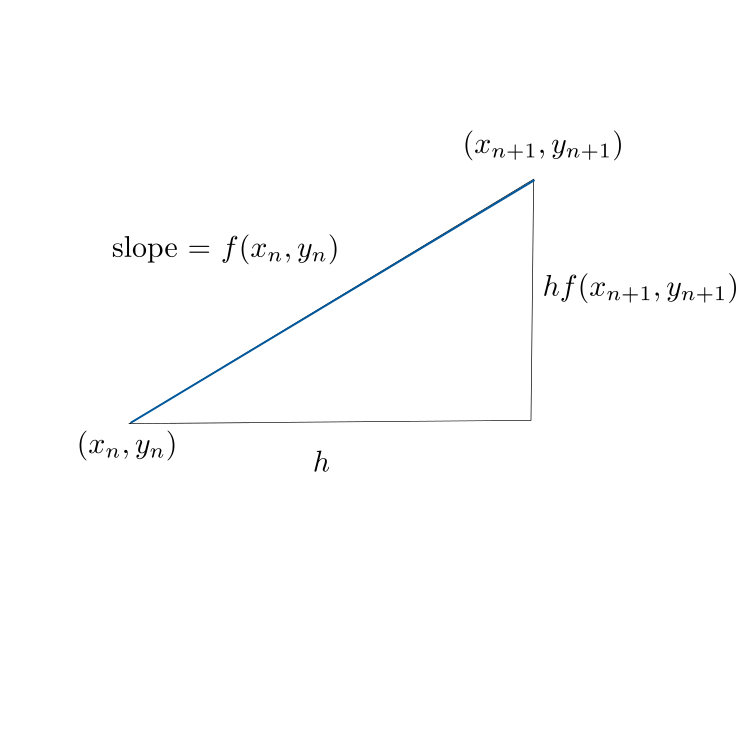
\includegraphics[scale=.3]{euler2}
  \end{flushleft}
  \( h = x_1-x_0 \)
  \[ y = f(x_0, y_0)(x-x_0) + y_0 \implies \]
  \[ y_1 = f(x_0, y_0)h + y_0 \]
  In general, 
  \[ \boxed{ y_{n+1} = hf(x_n,y_n) + y_n} \]
  Here
  \[ \boxed{ y_n \approx y(x_n)} \]
  % }}}

  % Date: 03.11.15 ------------------ {{{
  \newpage
  \marginpar{Date: 03.11.15 }
  Recall that an nth order linear ODE has the form 
  \[ 
  \tag{1} 
  \label{nth order linear ODE}
  y^{(n)} + \sum_{k=1}^n Pk(x)y^{(n-k)} = f(x)
  \]
  where \( Pk \) and \( f \) are cts for \( 1 \leq k \leq n \). \\
  The associated homogeneous nth order linear ODE to (1) is\\
  (2)
  \[ y^{(n)} + \sum_{k=1}^n Pk(x)y^{(n-k)} = 0 \]
  i.e., (1) with \( f(x) \equiv 0 \)\\
  Notation. put 
  \[ V = { y: I \to \mathbb{R} \text{ |  y has nth order derivative on I}  } \]
  then \( V \) is an \( \mathbb{R} \)- linear space. put 
  \[ W =  { y \in V \text{ | y is a soln to (2) }  } \]
  then the following holds\\[5mm]
  thrm. \( W \leq V \), i.e., the set of all solns to (2) is a linear
  space. \\
  Proof. If \( y \in W \) \& \( c \in \mathbb{R} \) then 
  \[ (cy)^{(n)} + \sum_{k=1}^n Pk(x)(cy)^{(n-k)}  = \]
  \[ (cy)^{(n)} + c\sum_{k=1}^n Pk(x)y^{(n-k)} \]
  \[ c(y^{(n)} + \sum_{k=1}^n Pk(x)y^{(n-k)}) \]
  \[ c \cdot 0 = 0 \]
  \( \therefore cy\in W \) \\
  If \( y_1, y_2 \in W \) then 
  \[ (y_1 + y_2)^{(n)} + \sum_{k=1}^n Pk(x)(y_1 +y_2 )^{(n-k)} = \]
  \[ y_1^{(n)} + \sum_{k=1}^n Pk(x)y_1^{(n-k)} + y_2^{(n)} +
  \sum_{k=1}^n Pk(x)y_2^{(n-k)} = \]
  \[ 0 + 0 = 0  \]
  \( \therefore y_1 + y_2 \in W \). Hence, \( W \in \mathbb{R} \)-linear
  subspace of V. \\[5mm]
  Recall: 
  Thrm (wronskian thrm). if \( f_1, ..., f_n \) are linearly independent
  in \( c^{(n-1)} (I) = \{ f:I\to \mathbb{R} \text{ | } f^{(n-1)} \text{
  is cts on I} \} \), then the wronskian of \( f_1, ..., f_n \) is identically 0
  for all \( x \in I \), i.e., for all \( x \in I \), 

  \[ |W(f_1, ...,f_n)(x)|  = det 
  \begin{pmatrix} 
    f_1(x)         & \cdots & f_n(x) \\
    f_1'(x)        & \cdots & f_n'(x) \\
    f_1''(x)       & \cdots & f_n''(x) \\
    \vdots         & \ddots & \vdots\\
    f_1^{(n-1)}(x) & \cdots & f_n^{(n-1)}(x) \\
  \end{pmatrix}
  =0\]


  Aside
  \[ A \vec{x}  = \vec{b} \]
  the soln space of 
  \[ A \vec{x} =\vec{0} \]
  is a linear space. the soln space of 
  \[ A \vec{x}  = \vec{b} \]
  is a affine linear space, with solns 
  \[ \vec{x} = \vec{x_0} + \vec{x_1}\]
  where \( \vec{x_0} \) is any hom soln

\section*{Exam 2}
  1. hom ODE \\
  2. ODE needing a subst to reduse to a 1st order linear/sep \\
  3. exact ODE \\
  4. population Model (logistic pop) \\
  5. population Model (havesting a logistic pop) \\ 
  % }}}

  % side stuff --------------- {{{
  %\section{Date: 02:18:2015}
  %Books \\
  %enderton "Mathematical logic" \\
  %kurnen "set theory" \\
  % Shellah's Archive
  % }}}

  %xy-pic
  %asymptote 


  \end{document}
